\newcommand{\titulus}{\nomenFesti{S. Callisti I, Papæ \& Martyris.}
\dies{Die 14. Octobris.}}
\newcommand{\oratio}{\pars{Oratio.}

\noindent Preces pópuli tui, quǽsumus, Dómine, cleménter exáudi, ut beáti Callísti, papæ, méritis adiuvémur, cuius passióne lætámur.

\pars{Pro pace in Ucraina.} \scriptura{Sir. 50, 25; 2 Esdr. 4, 20; \textbf{H416}}

\vspace{-4mm}

\antiphona{II D}{temporalia/ant-dapacemdomine.gtex}

\vfill

\noindent Deus, a quo sancta desidéria, recta consília et iusta sunt ópera: da servis tuis illam, quam mundus dare non potest, pacem; ut et corda nostra mandátis tuis dédita, et hóstium subláta formídine, témpora sint tua protectióne tranquílla.

\noindent Per Dóminum nostrum Iesum Christum, Fílium tuum, qui tecum vivit et regnat in unitáte Spíritus Sancti, Deus, per ómnia sǽcula sæculórum.

\noindent \Rbardot{} Amen.}
\newcommand{\invitatorium}{\pars{Invitatorium.}

\vspace{-4mm}

\antiphona{E}{temporalia/inv-regemmartyrumsimplex.gtex}}
\newcommand{\hymnusmatutinum}{\pars{Hymnus}

\cuminitiali{I}{temporalia/hym-BeateMartyr.gtex}}
\newcommand{\matversus}{\noindent \Vbardot{} Fili mi, atténde ad sapiéntiam meam.

\noindent \Rbardot{} Et prudéntiæ meæ inclína aurem tuam.}
\newcommand{\lectioi}{\pars{Lectio I.} \scriptura{Mal. 1, 10-14; 2, 13-16}

\noindent Incipit liber Malachíæ prophétæ.

\noindent Verbum Dómini ad Israel in manu Malachíæ.

\noindent «Diléxi vos, dicit Dóminus, et dixístis: “In quo dilexísti nos?”. Nonne frater erat Esau Iacob?, dicit Dóminus; et diléxi Iacob, Esau autem ódio hábui et pósui montes eius in solitúdinem et hereditátem eius thóibus desérti. Quod si díxerit Edom: “Destrúcti sumus, sed reverténtes ædificábimus, quæ destrúcta sunt”, hæc dicit Dóminus exercítuum: Isti ædificábunt, et ego déstruam; et vocabúntur ‘Términi impietátis’ et ‘Pópulus, cui irátus est Dóminus usque in ætérnum’. Et óculi vestri vidébunt et vos dicétis: “Magnificátus est Dóminus ultra términos Israel”.

\noindent Fílius honórat patrem et servus dóminum suum. Si ergo pater ego sum, ubi est honor meus? Et si Dóminus ego sum, ubi est timor meus?, dicit Dóminus exercítuum ad vos, o sacerdótes, qui despícitis nomen meum et dícitis: “In quo despéximus nomen tuum?”. Offértis super altáre meum panem pollútum et dícitis: “In quo pollúimus te?”. In eo quod dícitis: “Mensa Dómini contemptíbilis est”. Si offerátis cæcum ad immolándum, nonne malum est? Et si offerátis claudum et lánguidum, nonne malum est? Offer illud duci tuo, si placúerit ei aut si suscéperit fáciem tuam!, dicit Dóminus exercítuum. Sed nunc deprecámini vultum Dei, ut misereátur vestri! De manu enim vestra factum est hoc. Num suscípiet fácies vestras?, dicit Dóminus exercítuum.

\noindent Quis est in vobis, qui claudat óstia, ne incendátis altáre meum gratuíto? Non est mihi volúntas in vobis, dicit Dóminus exercítuum; et munus non suscípiam de manu vestra. Ab ortu enim solis usque ad occásum magnum est nomen meum in géntibus, et in omni loco sacrificátur et offértur nómini meo oblátio munda, quia magnum nomen meum in géntibus, dicit Dóminus exercítuum.

\noindent {\color{gray} Vos autem polluístis illud in eo quod dícitis: “Mensa Dómini contamináta est, et contemptíbilis esca eius”. Et dícitis: “Quantus labor!”, et despícitis illam, dicit Dóminus exercítuum. Et infértis de rapínis claudum et lánguidum et infértis sicut munus. Numquid suscípiam illud de manu vestra?, dicit Dóminus. Maledíctus dolósus, qui habet in grege suo másculum et votum fáciens ímmolat débile Dómino. Quia Rex magnus ego, dicit Dóminus exercítuum, et nomen meum horríbile in géntibus.

\noindent Et hoc rursum fácitis: operítis lácrimis altáre Dómini, fletu et mugítu, ita ut non respíciam ultra ad sacrifícium nec accípiam placábile quid de manu vestra; et dícitis: “Quam ob causam?”. Quia Dóminus testificátus est inter te et uxórem adulescéntiæ tuæ, cui tu factus es infidélis; et hæc párticeps tua et uxor fœ́deris tui. Nonne unitátem fecit carnis et spíritus? Et quid únitas quærit nisi semen a Deo? Custodíte ergo spíritum vestrum; et uxóri adulescéntiæ tuæ noli esse infidélis. Si quis ódio dimíttit, dicit Dóminus, Deus Israel, óperit iníquitas vestiméntum eius, dicit Dóminus exercítuum. Custodíte spíritum vestrum et nolíte esse infidéles.»}}
\newcommand{\responsoriumi}{\pars{Responsorium 1.} \scriptura{\Rbardot{} Ps. 112, 3 \Vbardot{} ibid., 4; \textbf{H92}}

\vspace{-5mm}

\responsorium{VIII}{temporalia/resp-asolisortu-CROCHU.gtex}{}}
\newcommand{\lectioii}{\pars{Lectio II.} \scriptura{Cap. 13: CSEL 3, 346-347}

\noindent Ex Tractátu sancti Cypriáni epíscopi et mártyris ad Fortunátum.

\noindent \emph{Non sunt condígnæ passiónes huius témporis ad superventúram claritúdinem quæ revelábitur in nobis.} Quis ergo non ómnibus modis elabóret ad claritátem tantam perveníre, ut amícus Dei fiat, ut cum Christo statim gáudeat, ut post torménta et supplícia terréna prǽmia divína percípiat? Si milítibus sæculáribus gloriósum est ut hoste devícto rédeant in pátriam triumphántes, quanto pótior et maior est glória victo diábolo ad paradísum triumphántem redíre et, unde Adam peccátor eiéctus est, illuc prostráto eo qui ante decéperat tropǽa victrícia reportáre, offérre Dómino acceptíssimum munus incorrúptam fidem, virtútem mentis incólumem, laudem devotiónis illústrem, comitári eum cum veníre cœ́perit vindíctam de inimícis receptúrus, láteri eius assístere cum séderit iudicatúrus, coherédem Christi fíeri, ángelis coæquári, cum patriárchis, cum apóstolis, cum prophétis cæléstis regni possessióne lætári.}
\newcommand{\responsoriumii}{\pars{Responsorium 2.} \scriptura{\textbf{H373}}

\vspace{-5mm}

\responsorium{III}{temporalia/resp-istecognovit-CROCHU.gtex}{}

\vfill
\pagebreak

\rubrica{vel ad libitum:}

\vspace{3mm}

\pars{Responsorium 2.}

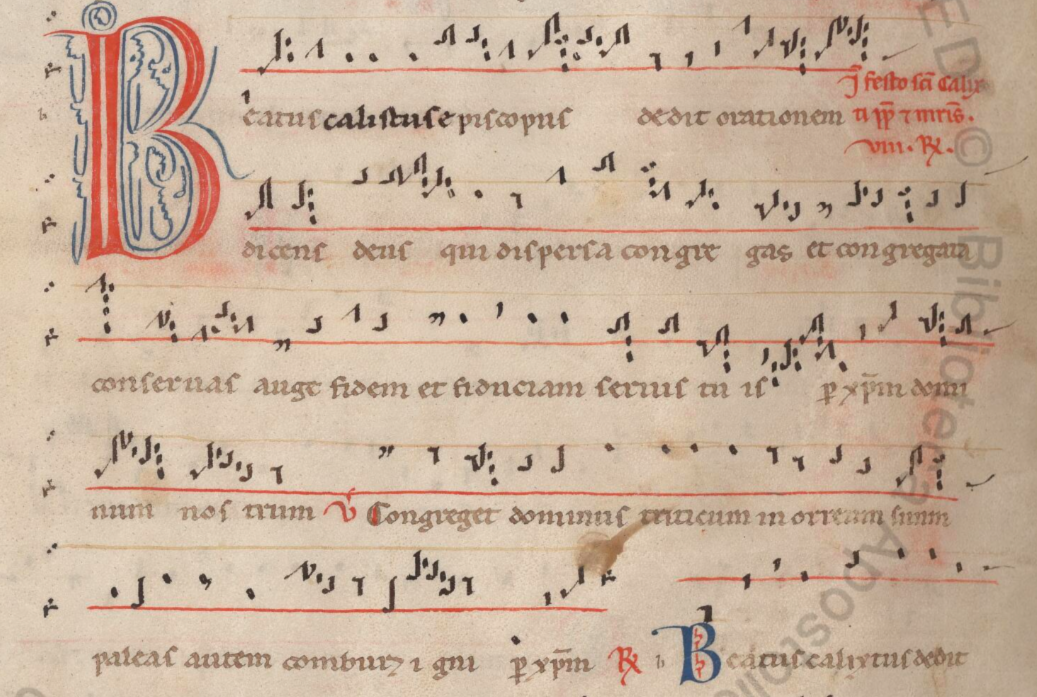
\includegraphics[width=17cm]{pic-beatuscallistus.png}}
\newcommand{\lectioiii}{\pars{Lectio III.}

\noindent Has cogitatiónes quæ persecútio potest víncere, quæ possunt torménta superáre? Durat fortis et stábilis religiósis meditatiónibus fundáta mens et advérsus omnes diáboli terróres et minas mundi ánimus immóbilis perstat, quem futurórum fides certa et sólida corróborat. Claudúntur in persecutiónibus terræ, sed patet cælum; minátur antichrístus, sed Christus tuétur; mors infértur, sed immortálitas séquitur. Quanta est dígnitas et quanta secúritas exíre hinc lætum, exíre inter pressúras et angústias gloriósum, cláudere in moménto óculos, quibus hómines videbántur et mundus, aperíre eósdem statim, ut Deus videátur et Christus. Tam felíciter migrándi quanta velócitas. Terris repénte subtráheris, ut in regnis cæléstibus reponáris.

\noindent Hæc opórtet mente et cogitatióne complécti, hæc die ac nocte meditári. Si talem persecútio invénerit Dei mílitem, vinci non póterit virtus ad prœ́lium prompta. Vel si arcessítio ante prævénerit, sine prǽmio non erit fides quæ erat ad martýrium præparáta; sine damno témporis merces Deo iúdice rédditur; in persecutióne milítia, in pace consciéntia coronátur.}
\newcommand{\responsoriumiii}{\pars{Responsorium 3.} \scriptura{\Rbardot{} Ps. 8, 6-8 \Vbardot{} Ps. 20, 4; \textbf{H374}}

\vspace{-5mm}

\responsorium{VII}{temporalia/resp-gloriaethonore-CROCHU-cumdox.gtex}{}}
\newcommand{\hymnuslaudes}{\pars{Hymnus}

\cuminitiali{VI}{temporalia/hym-MartyrDei.gtex}}
\newcommand{\lectiobrevis}{\pars{Lectio Brevis.} \scriptura{2 Cor. 1, 3-5}

\noindent Benedíctus Deus et Pater Dómini nostri Iesu Christi, Pater misericordiárum et Deus totíus consolatiónis, qui consolátur nos in omni tribulatióne nostra, ut possímus et ipsi consolári eos, qui in omni pressúra sunt, per exhortatiónem, qua exhortámur et ipsi a Deo; quóniam, sicut abúndant passiónes Christi in nobis, ita per Christum abúndat et consolátio.}
\newcommand{\responsoriumbreve}{\pars{Responsorium breve.} \scriptura{Ex. 15, 2}

\cuminitiali{VI}{temporalia/resp-fortitudomeaetlausmea.gtex}}
\newcommand{\preces}{\noindent Fratres, Salvatórem nostrum, testem fidélem, per mártyres interféctos propter verbum Dei,~\gredagger{} celebrémus, clamántes:

\Rbardot{} Redemísti nos Deo in sánguine tuo.

\noindent Per mártyres tuos, qui líbere mortem in testimónium fídei sunt ampléxi,~\gredagger{} da nobis, Dómine, veram spíritus libertátem.

\Rbardot{} Redemísti nos Deo in sánguine tuo.

\noindent Per mártyres tuos, qui fidem usque ad sánguinem sunt conféssi,~\gredagger{} da nobis, Dómine, puritátem fideíque constántiam.

\Rbardot{} Redemísti nos Deo in sánguine tuo.

\noindent Per mártyres tuos, qui, sustinéntes crucem, tua vestígia sunt secúti,~\gredagger{} da nobis, Dómine, ærúmnas vitæ fórtiter sustinére.

\Rbardot{} Redemísti nos Deo in sánguine tuo.

\noindent Per mártyres tuos, qui stolas suas lavérunt in sánguine Agni,~\gredagger{} da nobis, Dómine, omnes insídias carnis mundíque devíncere.

\Rbardot{} Redemísti nos Deo in sánguine tuo.}
\newcommand{\benedictus}{\pars{Canticum Zachariæ.} \scriptura{Io. 12, 35; \textbf{H375}}

\vspace{-4mm}

\antiphona{III a}{temporalia/ant-quisequiturmenonambulat.gtex}

%\vspace{-2mm}

\scriptura{Lc. 1, 68-79}

\vspace{-2mm}

\cantusSineNeumas
\initiumpsalmi{temporalia/benedictus-initium-iii-a-auto.gtex}

%\vspace{-1.5mm}

\input{temporalia/benedictus-iii-a.tex} \Abardot{}}
\newcommand{\precestotum}{\pars{Deprecatio Gelasii}

\vspace{-5mm}

\grechangedim{interwordspacetext}{0.16 cm plus 0.15 cm minus 0.05 cm}{scalable}%
\antiphona{D\textsuperscript{1}}{temporalia/deprecatio4-propace.gtex}
\grechangedim{interwordspacetext}{0.22 cm plus 0.15 cm minus 0.05 cm}{scalable}%

\vfill

\pars{Oratio Dominica.}

\cuminitiali{D}{temporalia/oratiodominica-d.gtex}}
\newcommand{\dominusnosbenedicat}{\antiphona{D}{temporalia/dominusnosbenedicat-d.gtex}}
\newcommand{\benedicamuslaudes}{\cuminitiali{}{temporalia/benedicamus-memoria-laudes.gtex}}
\newcommand{\hebdomada}{infra Hebdom. XXVIII per Annum.}
%\newcommand{\hiemalis}{Hiemalis}
\newcommand{\matud}{Matutinum Hebdomadae D}
\newcommand{\matubd}{Matutinum Hebdomadae B vel D}
\newcommand{\laudd}{Laudes Hebdomadae D}
\newcommand{\laudbd}{Laudes Hebdomadae B vel D}

% LuaLaTeX

\documentclass[a4paper, twoside, 12pt]{article}
\usepackage[latin]{babel}
%\usepackage[landscape, left=3cm, right=1.5cm, top=2cm, bottom=1cm]{geometry} % okraje stranky
%\usepackage[landscape, a4paper, mag=1166, truedimen, left=2cm, right=1.5cm, top=1.6cm, bottom=0.95cm]{geometry} % okraje stranky
\usepackage[landscape, a4paper, mag=1400, truedimen, left=0.5cm, right=0.5cm, top=0.5cm, bottom=0.5cm]{geometry} % okraje stranky

\usepackage{fontspec}
\setmainfont[FeatureFile={junicode.fea}, Ligatures={Common, TeX}, RawFeature=+fixi]{Junicode}
%\setmainfont{Junicode}

% shortcut for Junicode without ligatures (for the Czech texts)
\newfontfamily\nlfont[FeatureFile={junicode.fea}, Ligatures={Common, TeX}, RawFeature=+fixi]{Junicode}

\usepackage{multicol}
\usepackage{color}
\usepackage{lettrine}
\usepackage{fancyhdr}

% usual packages loading:
\usepackage{luatextra}
\usepackage{graphicx} % support the \includegraphics command and options
\usepackage{gregoriotex} % for gregorio score inclusion
\usepackage{gregoriosyms}
\usepackage{wrapfig} % figures wrapped by the text
\usepackage{parcolumns}
\usepackage[contents={},opacity=1,scale=1,color=black]{background}
\usepackage{tikzpagenodes}
\usepackage{calc}
\usepackage{longtable}
\usetikzlibrary{calc}

\setlength{\headheight}{14.5pt}

% Commands used to produce a typical "Conventus" booklet

\newenvironment{titulusOfficii}{\begin{center}}{\end{center}}
\newcommand{\dies}[1]{#1

}
\newcommand{\nomenFesti}[1]{\textbf{\Large #1}

}
\newcommand{\celebratio}[1]{#1

}

\newcommand{\hora}[1]{%
\vspace{0.5cm}{\large \textbf{#1}}

\fancyhead[LE]{\thepage\ / #1}
\fancyhead[RO]{#1 / \thepage}
\addcontentsline{toc}{subsection}{#1}
}

% larger unit than a hora
\newcommand{\divisio}[1]{%
\begin{center}
{\Large \textsc{#1}}
\end{center}
\fancyhead[CO,CE]{#1}
\addcontentsline{toc}{section}{#1}
}

% a part of a hora, larger than pars
\newcommand{\subhora}[1]{
\begin{center}
{\large \textit{#1}}
\end{center}
%\fancyhead[CO,CE]{#1}
\addcontentsline{toc}{subsubsection}{#1}
}

% rubricated inline text
\newcommand{\rubricatum}[1]{\textit{#1}}

% standalone rubric
\newcommand{\rubrica}[1]{\vspace{3mm}\rubricatum{#1}}

\newcommand{\notitia}[1]{\textcolor{red}{#1}}

\newcommand{\scriptura}[1]{\hfill \small\textit{#1}}

\newcommand{\translatioCantus}[1]{\vspace{1mm}%
{\noindent\footnotesize \nlfont{#1}}}

% pruznejsi varianta nasledujiciho - umoznuje nastavit sirku sloupce
% s prekladem
\newcommand{\psalmusEtTranslatioB}[3]{
  \vspace{0.5cm}
  \begin{parcolumns}[colwidths={2=#3}, nofirstindent=true]{2}
    \colchunk{
      \input{#1}
    }

    \colchunk{
      \vspace{-0.5cm}
      {\footnotesize \nlfont
        \input{#2}
      }
    }
  \end{parcolumns}
}

\newcommand{\psalmusEtTranslatio}[2]{
  \psalmusEtTranslatioB{#1}{#2}{8.5cm}
}


\newcommand{\canticumMagnificatEtTranslatio}[1]{
  \psalmusEtTranslatioB{#1}{temporalia/extra-adventum-vespers/magnificat-boh.tex}{12cm}
}
\newcommand{\canticumBenedictusEtTranslatio}[1]{
  \psalmusEtTranslatioB{#1}{temporalia/extra-adventum-laudes/benedictus-boh.tex}{10.5cm}
}

% volne misto nad antifonami, kam si zpevaci dokresli neumy
\newcommand{\hicSuntNeumae}{\vspace{0.5cm}}

% prepinani mista mezi notovymi osnovami: pro neumovane a neneumovane zpevy
\newcommand{\cantusCumNeumis}{
  \setgrefactor{17}
  \global\advance\grespaceabovelines by 5mm%
}
\newcommand{\cantusSineNeumas}{
  \setgrefactor{17}
  \global\advance\grespaceabovelines by -5mm%
}

% znaky k umisteni nad inicialu zpevu
\newcommand{\superInitialam}[1]{\gresetfirstlineaboveinitial{\small {\textbf{#1}}}{\small {\textbf{#1}}}}

% pars officii, i.e. "oratio", ...
\newcommand{\pars}[1]{\textbf{#1}}

\newenvironment{psalmus}{
  \setlength{\parindent}{0pt}
  \setlength{\parskip}{5pt}
}{
  \setlength{\parindent}{10pt}
  \setlength{\parskip}{10pt}
}

%%%% Prejmenovat na latinske:
\newcommand{\nadpisZalmu}[1]{
  \hspace{2cm}\textbf{#1}\vspace{2mm}%
  \nopagebreak%

}

% mode, score, translation
\newcommand{\antiphona}[3]{%
\hicSuntNeumae
\superInitialam{#1}
\includescore{#2}

#3
}
 % Often used macros

\newcommand{\annusEditionis}{2021}

%%%% Vicekrat opakovane kousky

\newcommand{\anteOrationem}{
  \rubrica{Ante Orationem, cantatur a Superiore:}

  \pars{Supplicatio Litaniæ.}

  \cuminitiali{}{temporalia/supplicatiolitaniae.gtex}

  \pars{Oratio Dominica.}

  \cuminitiali{}{temporalia/oratiodominica.gtex}

  \rubrica{Deinde dicitur ab Hebdomadario:}

  \cuminitiali{}{temporalia/dominusvobiscum-solemnis.gtex}

  \rubrica{In choro monialium loco Dominus vobiscum dicitur:}

  \sineinitiali{temporalia/domineexaudi.gtex}
}

\setlength{\columnsep}{30pt} % prostor mezi sloupci

%%%%%%%%%%%%%%%%%%%%%%%%%%%%%%%%%%%%%%%%%%%%%%%%%%%%%%%%%%%%%%%%%%%%%%%%%%%%%%%%%%%%%%%%%%%%%%%%%%%%%%%%%%%%%
\begin{document}

% Here we set the space around the initial.
% Please report to http://home.gna.org/gregorio/gregoriotex/details for more details and options
\grechangedim{afterinitialshift}{2.2mm}{scalable}
\grechangedim{beforeinitialshift}{2.2mm}{scalable}
\grechangedim{interwordspacetext}{0.22 cm plus 0.15 cm minus 0.05 cm}{scalable}%
\grechangedim{annotationraise}{-0.2cm}{scalable}

% Here we set the initial font. Change 38 if you want a bigger initial.
% Emit the initials in red.
\grechangestyle{initial}{\color{red}\fontsize{38}{38}\selectfont}

\pagestyle{empty}

%%%% Titulni stranka
\begin{titulusOfficii}
\ifx\titulus\undefined
\nomenFesti{Feria VI \hebdomada{}}
\else
\titulus
\fi
\end{titulusOfficii}

\vfill

\begin{center}
%Ad usum et secundum consuetudines chori \guillemotright{}Conventus Choralis\guillemotleft.

%Editio Sancti Wolfgangi \annusEditionis
\end{center}

\scriptura{}

\pars{}

\pagebreak

\renewcommand{\headrulewidth}{0pt} % no horiz. rule at the header
\fancyhf{}
\pagestyle{fancy}

\cantusSineNeumas

\ifx\oratio\undefined
\ifx\lauda\undefined
\else
\newcommand{\oratio}{\pars{Oratio.}

\noindent Deus, qui ténebras ignorántiæ Verbi tui luce depéllis, auge in córdibus nostris virtútem fídei quam dedísti, ut ignis, quem grátia tua fecit accéndi, nullis tentatiónibus exstinguátur.

\noindent Per Dóminum nostrum Iesum Christum, Fílium tuum, qui tecum vivit et regnat in unitáte Spíritus Sancti, Deus, per ómnia sǽcula sæculórum.

\noindent \Rbardot{} Amen.}
\fi
\ifx\laudb\undefined
\else
\newcommand{\oratio}{\pars{Oratio.}

\noindent Præsta, quǽsumus, omnípotens Deus, ut laudes, quas nunc tibi persólvimus, in ætérnum cum sanctis tuis ubérius decantáre valeámus.

\noindent Per Dóminum nostrum Iesum Christum, Fílium tuum, qui tecum vivit et regnat in unitáte Spíritus Sancti, Deus, per ómnia sǽcula sæculórum.

\noindent \Rbardot{} Amen.}
\fi
\ifx\laudc\undefined
\else
\newcommand{\oratio}{\pars{Oratio.}

\noindent Illábere sénsibus nostris, omnípotens Pater, ut, in præceptórum tuórum lúmine gradiéntes, te ducem semper sequámur et príncipem.

\noindent Per Dóminum nostrum Iesum Christum, Fílium tuum, qui tecum vivit et regnat in unitáte Spíritus Sancti, Deus, per ómnia sǽcula sæculórum.

\noindent \Rbardot{} Amen.}
\fi
\fi

\hora{Ad Matutinum.} %%%%%%%%%%%%%%%%%%%%%%%%%%%%%%%%%%%%%%%%%%%%%%%%%%%%%

\vspace{2mm}

\cuminitiali{}{temporalia/dominelabiamea.gtex}

\vfill
%\pagebreak

\vspace{2mm}

\ifx\invitatorium\undefined
\pars{Invitatorium.} \scriptura{Ps. 94, 6.7; Psalmus 94}

\antiphona{E}{temporalia/inv-dominumdeum.gtex}
\else
\invitatorium
\fi

\vfill
\pagebreak

\ifx\hymnusmatutinum\undefined
\ifx\matuac\undefined
\else
\pars{Hymnus.} \scriptura{Gregorius Magnus (+604)}

{
\grechangedim{interwordspacetext}{0.10 cm plus 0.15 cm minus 0.05 cm}{scalable}%
\antiphona{IV}{temporalia/hym-TuTrinitatis.gtex}
\grechangedim{interwordspacetext}{0.22 cm plus 0.15 cm minus 0.05 cm}{scalable}%
}
\fi
\ifx\matubd\undefined
\else
\pars{Hymnus.}

{
\grechangedim{interwordspacetext}{0.10 cm plus 0.15 cm minus 0.05 cm}{scalable}%
\antiphona{II}{temporalia/hym-GalliCantu.gtex}
\grechangedim{interwordspacetext}{0.22 cm plus 0.15 cm minus 0.05 cm}{scalable}%
}
\fi
\else
\hymnusmatutinum
\fi

\vspace{-3mm}

\vfill
\pagebreak

\ifx\matua\undefined
\else
% MAT A
\pars{Psalmus 1.} \scriptura{Ps. 34, 1; \textbf{H93}}

\vspace{-4mm}

\antiphona{IV g}{temporalia/ant-expugnaimpugnantes.gtex}

%\vspace{-2mm}

\scriptura{Ps. 34, 1-10}

%\vspace{-2mm}

\initiumpsalmi{temporalia/ps34i-initium-iv-g-auto.gtex}

\input{temporalia/ps34i-iv-g.tex} \Abardot{}

\vfill
\pagebreak

\pars{Psalmus 2.} \scriptura{Ps. 118, 154; \textbf{H174}}

\vspace{-4mm}

\antiphona{VIII G}{temporalia/ant-iudicacausam.gtex}

%\vspace{-2mm}

\scriptura{Ps. 34, 11-17}

%\vspace{-2mm}

\initiumpsalmi{temporalia/ps34ii-initium-viii-G-auto.gtex}

\input{temporalia/ps34ii-viii-G.tex} \Abardot{}

\vfill
\pagebreak

\pars{Psalmus 3.} \scriptura{Ps. 50, 16; \textbf{H177}}

\vspace{-4mm}

\antiphona{VIII G}{temporalia/ant-liberame.gtex}

%\vspace{-2mm}

\scriptura{Ps. 34, 18-28}

\vspace{-2mm}

\initiumpsalmi{temporalia/ps34iii-initium-viii-G-auto.gtex}

\input{temporalia/ps34iii-viii-G.tex} \Abardot{}

\vfill
\pagebreak
\fi
\ifx\matub\undefined
\else
% MAT B
\pars{Psalmus 1.} \scriptura{Ps. 37, 2}

\vspace{-4mm}

\antiphona{VIII c}{temporalia/ant-neiniratua.gtex}

%\vspace{-2mm}

\scriptura{Ps. 37, 2-5}

%\vspace{-2mm}

\initiumpsalmi{temporalia/ps37ii_v-initium-viii-C-auto.gtex}

\input{temporalia/ps37ii_v-viii-C.tex} \Abardot{}

\vfill
\pagebreak

\pars{Psalmus 2.} \scriptura{Ps. 34, 4; \textbf{H218}}

\vspace{-4mm}

\antiphona{II* a}{temporalia/ant-confundantur.gtex}

%\vspace{-2mm}

\scriptura{Ps. 37, 6-13}

%\vspace{-2mm}

\initiumpsalmi{temporalia/ps37vi_xiii-initium-ii_-a-auto.gtex}

\input{temporalia/ps37vi_xiii-ii_-a.tex} \Abardot{}

\vfill
\pagebreak

\pars{Psalmus 3.} \scriptura{Ps. 139, 9.8}

\vspace{-4mm}

\antiphona{II A}{temporalia/ant-nederelinquasme.gtex}

%\vspace{-2mm}

\scriptura{Ps. 37, 14-23}

%\vspace{-2mm}

\initiumpsalmi{temporalia/ps37xiv_xxiii-initium-ii-A-auto.gtex}

\input{temporalia/ps37xiv_xxiii-ii-A.tex} \Abardot{}

\vfill
\pagebreak
\fi
\ifx\matuc\undefined
\else
% MAT C
\pars{Psalmus 1.} \scriptura{Ps. 68, 10; \textbf{H178}}

\vspace{-4mm}

\antiphona{VIII c}{temporalia/ant-zelusdomus.gtex}

%\vspace{-3mm}

\scriptura{Ps. 68, 2-13}

%\vspace{-2mm}

\initiumpsalmi{temporalia/ps68ii_xiii-initium-viii-c-auto.gtex}

%\vspace{-1.5mm}

\input{temporalia/ps68ii_xiii-viii-c.tex}

\vfill

\antiphona{}{temporalia/ant-zelusdomus.gtex}

\vfill
\pagebreak

\pars{Psalmus 2.}

\vspace{-4mm}

\antiphona{VIII c}{temporalia/ant-consolantemme.gtex}

%\vspace{-2mm}

\scriptura{Ps. 68, 14-22}

%\vspace{-2mm}

\initiumpsalmi{temporalia/ps68xiv_xxii-initium-viii-c-auto.gtex}

\input{temporalia/ps68xiv_xxii-viii-c.tex} \Abardot{}

\vfill
\pagebreak

\pars{Psalmus 3.} \scriptura{Ps. 68, 33; \textbf{H96}}

\vspace{-4mm}

\antiphona{VIII G}{temporalia/ant-quaeritedominumet.gtex}

%\vspace{-2mm}

\scriptura{Ps. 68, 30-37}

%\vspace{-2mm}

\initiumpsalmi{temporalia/ps68iii-initium-viii-G-auto.gtex}

\input{temporalia/ps68iii-viii-G.tex} \Abardot{}

\vfill
\pagebreak
\fi
\ifx\matud\undefined
\else
% MAT D
\pars{Psalmus 1.} \scriptura{Ps. 72, 8; \textbf{H179}}

\vspace{-4mm}

\antiphona{VIII c}{temporalia/ant-cogitaveruntimpii.gtex}

%\vspace{-3mm}

\scriptura{Ps. 54, 2-8}

%\vspace{-2mm}

\initiumpsalmi{temporalia/ps54i-initium-viii-c-auto.gtex}

%\vspace{-1.5mm}

\input{temporalia/ps54i-viii-c.tex} \Abardot{}

\vfill
\pagebreak

\pars{Psalmus 2.} \scriptura{Ps. 34, 4; \textbf{H178}}

\vspace{-4mm}

\antiphona{VII c\textsuperscript{2}}{temporalia/ant-avertanturretrorsum.gtex}

%\vspace{-2mm}

\scriptura{Ps. 54, 9-16}

%\vspace{-2mm}

\initiumpsalmi{temporalia/ps54ii-initium-vii-c2-auto.gtex}

\input{temporalia/ps54ii-vii-c2.tex} \Abardot{}

\vfill
\pagebreak

\pars{Psalmus 3.}

\vspace{-4mm}

\antiphona{VIII G}{temporalia/ant-iustusnonconturbabitur.gtex}

%\vspace{-2mm}

\scriptura{Ps. 54, 17-24}

%\vspace{-2mm}

\initiumpsalmi{temporalia/ps54iii-initium-viii-G-auto.gtex}

\input{temporalia/ps54iii-viii-G.tex} \Abardot{}

\vfill
\pagebreak
\fi

\pars{Versus.}

\ifx\matversus\undefined
\ifx\matua\undefined
\else
\noindent \Vbardot{} Fili mi, custódi sermónes meos.

\noindent \Rbardot{} Serva mandáta mea et vives.
\fi
\ifx\matub\undefined
\else
\noindent \Vbardot{} Oculi mei defecérunt in desidério salutáris tui.

\noindent \Rbardot{} Et elóquii iustítiæ tuæ.
\fi
\ifx\matuc\undefined
\else
\noindent \Vbardot{} Dóminus vias suas docébit nos.

\noindent \Rbardot{} Et ambulábimus in sémitis eius.
\fi
\ifx\matud\undefined
\else
\noindent \Vbardot{} Tribulátio et angústia invenérunt me.

\noindent \Rbardot{} Mandáta tua meditátio mea est.
\fi
\else
\matversus
\fi

\vspace{5mm}

\sineinitiali{temporalia/oratiodominica-mat.gtex}

\vspace{5mm}

\pars{Absolutio.}

\cuminitiali{}{temporalia/absolutio-ipsius.gtex}

\vfill
\pagebreak

\cuminitiali{}{temporalia/benedictio-solemn-deus.gtex}

\vspace{7mm}

\lectioi

\noindent \Vbardot{} Tu autem, Dómine, miserére nobis.
\noindent \Rbardot{} Deo grátias.

\vfill
\pagebreak

\responsoriumi

\vfill
\pagebreak

\cuminitiali{}{temporalia/benedictio-solemn-christus.gtex}

\vspace{7mm}

\lectioii

\noindent \Vbardot{} Tu autem, Dómine, miserére nobis.
\noindent \Rbardot{} Deo grátias.

\vfill
\pagebreak

\responsoriumii

\vfill
\pagebreak

\cuminitiali{}{temporalia/benedictio-solemn-ignem.gtex}

\vspace{7mm}

\lectioiii

\noindent \Vbardot{} Tu autem, Dómine, miserére nobis.
\noindent \Rbardot{} Deo grátias.

\vfill
\pagebreak

\responsoriumiii

\vfill
\pagebreak

\rubrica{Reliqua omittuntur, nisi Laudes separandæ sint.}

\sineinitiali{temporalia/domineexaudi.gtex}

\vfill

\oratio

\vfill

\noindent \Vbardot{} Dómine, exáudi oratiónem meam.
\Rbardot{} Et clamor meus ad te véniat.

\vfill

\noindent \Vbardot{} Benedicámus Dómino.
\noindent \Rbardot{} Deo grátias.

\vfill

\noindent \Vbardot{} Fidélium ánimæ per misericórdiam Dei requiéscant in pace.
\Rbardot{} Amen.

\vfill
\pagebreak

\hora{Ad Laudes.} %%%%%%%%%%%%%%%%%%%%%%%%%%%%%%%%%%%%%%%%%%%%%%%%%%%%%

\cantusSineNeumas

\vspace{0.5cm}
\grechangedim{interwordspacetext}{0.18 cm plus 0.15 cm minus 0.05 cm}{scalable}%
\cuminitiali{}{temporalia/deusinadiutorium-communis-quad.gtex}
\grechangedim{interwordspacetext}{0.22 cm plus 0.15 cm minus 0.05 cm}{scalable}%

\vfill
\pagebreak

\ifx\hymnuslaudes\undefined
\ifx\laudac\undefined
\else
\pars{Hymnus}

\grechangedim{interwordspacetext}{0.16 cm plus 0.15 cm minus 0.05 cm}{scalable}%
\cuminitiali{I}{temporalia/hym-AEternaCaeli.gtex}
\grechangedim{interwordspacetext}{0.22 cm plus 0.15 cm minus 0.05 cm}{scalable}%
\vspace{-3mm}
\fi
\ifx\laudbd\undefined
\else
\pars{Hymnus}

\grechangedim{interwordspacetext}{0.16 cm plus 0.15 cm minus 0.05 cm}{scalable}%
\cuminitiali{IV}{temporalia/hym-DeusQui.gtex}
\grechangedim{interwordspacetext}{0.22 cm plus 0.15 cm minus 0.05 cm}{scalable}%
\vspace{-3mm}
\fi
\else
\hymnuslaudes
\fi

\vfill
\pagebreak

\ifx\lauda\undefined
\else
\pars{Psalmus 1.} \scriptura{Ps. 50, 3; \textbf{H93}}

\vspace{-4mm}

\antiphona{VI F}{temporalia/ant-misereremeideus.gtex}

\scriptura{Psalmus 50.}

\initiumpsalmi{temporalia/ps50-initium-vi-F-auto.gtex}

\input{temporalia/ps50-vi-F.tex}

\vfill

\antiphona{}{temporalia/ant-misereremeideus.gtex}

\vfill
\pagebreak

\pars{Psalmus 2.} \scriptura{Is. 45, 25}

\vspace{-4mm}

\antiphona{V a}{temporalia/ant-indominoiustificabitur.gtex}

\scriptura{Canticum Isaiæ, Is. 45, 15-30}

%\vspace{-2mm}

\initiumpsalmi{temporalia/isaiae2-initium-v-a-auto.gtex}

\input{temporalia/isaiae2-v-a.tex}

\vfill

\antiphona{}{temporalia/ant-indominoiustificabitur.gtex}

\vfill
\pagebreak

\pars{Psalmus 3.} \scriptura{Ps. 99, 1; \textbf{H98}}

\vspace{-4mm}

\antiphona{IV* e}{temporalia/ant-iubilatedeo.gtex}

\scriptura{Psalmus 99.}

\initiumpsalmi{temporalia/ps99-initium-iv_-e-auto.gtex}

\input{temporalia/ps99-iv_-e.tex} \Abardot{}

\vfill
\pagebreak
\fi
\ifx\laudb\undefined
\else
\pars{Psalmus 1.} \scriptura{Ps. 50, 4; \textbf{H95}}

\vspace{-4mm}

\antiphona{VII a}{temporalia/ant-ampliuslavame.gtex}

\scriptura{Psalmus 50.}

\initiumpsalmi{temporalia/ps50-initium-vii-a-auto.gtex}

\input{temporalia/ps50-vii-a.tex}

\vfill

\antiphona{}{temporalia/ant-ampliuslavame.gtex}

\vfill
\pagebreak

\pars{Psalmus 2.} \scriptura{Hab. 3, 2; \textbf{H99}}

\vspace{-6mm}

\antiphona{IV* e}{temporalia/ant-domineaudivi.gtex}

\vspace{-2mm}

\scriptura{Canticum Habacuc, Hab. 3, 2-19}

%\vspace{-2mm}

%\initiumpsalmi{temporalia/habacuc-initium-iv_-e-auto.gtex}
\initiumpsalmi{temporalia/habacuc-initium-iv_-e.gtex}

\input{temporalia/habacuc-iv_-e.tex}

\vfill

\antiphona{}{temporalia/ant-domineaudivi.gtex}

\vfill
\pagebreak

\pars{Psalmus 3.} \scriptura{Ps. 147, 12}

\vspace{-4mm}

\antiphona{E}{temporalia/ant-laudaierusalem.gtex}

\vspace{-2mm}

\scriptura{Psalmus 147.}

%\vspace{-3mm}

%\initiumpsalmi{temporalia/ps147-initium-e-auto.gtex}
\initiumpsalmi{temporalia/ps147-initium-e.gtex}

\input{temporalia/ps147-e.tex} \Abardot{}

\vfill
\pagebreak
\fi
\ifx\laudc\undefined
\else
\pars{Psalmus 1.} \scriptura{Ps. 50, 6.3; \textbf{H96}}

\vspace{-4mm}

\antiphona{VIII G\textsuperscript{2}}{temporalia/ant-tibisoli.gtex}

\scriptura{Psalmus 50.}

\initiumpsalmi{temporalia/ps50-initium-viii-G2-auto.gtex}

\input{temporalia/ps50-viii-G2.tex}

\vfill

\antiphona{}{temporalia/ant-tibisoli.gtex}

\vfill
\pagebreak

\pars{Psalmus 2.}

\vspace{-4mm}

\antiphona{VIII G}{temporalia/ant-nosnosderelinquas.gtex}

%\vspace{-2mm}

\scriptura{Canticum Ieremiæ, Ier. 14, 17-31}

%\vspace{-2mm}

\initiumpsalmi{temporalia/jeremiae2-initium-viii-G.gtex}

\input{temporalia/jeremiae2-viii-G.tex} \Abardot{}

\vfill
\pagebreak

\pars{Psalmus 3.}

\vspace{-4mm}

\antiphona{E}{temporalia/ant-servitedominoinlaetitia.gtex}

\vspace{-2mm}

\scriptura{Psalmus 99.}

%\vspace{-2mm}

\initiumpsalmi{temporalia/ps99-initium-e.gtex}

\input{temporalia/ps99-e.tex} \Abardot{}

\vfill
\pagebreak
\fi
\ifx\laudd\undefined
\else
\pars{Psalmus 1.} \scriptura{Ps. 50, 12}

\vspace{-4mm}

\antiphona{I a\textsuperscript{2}}{temporalia/ant-cormundumcrea.gtex}

\scriptura{Psalmus 50.}

\initiumpsalmi{temporalia/ps50-initium-i-a2-auto.gtex}

\input{temporalia/ps50-i-a2.tex}

\vfill

\antiphona{}{temporalia/ant-cormundumcrea.gtex}

\vfill
\pagebreak

\pars{Psalmus 2.}

\vspace{-4mm}

\antiphona{II D}{temporalia/ant-aedificansierusalem.gtex}

%\vspace{-2mm}

\scriptura{Canticum Tobiæ, Tob. 13, 10-18}

%\vspace{-2mm}

\initiumpsalmi{temporalia/tobiae2-initium-ii-D-auto.gtex}

\input{temporalia/tobiae2-ii-D.tex} \Abardot{}

\vfill
\pagebreak

\pars{Psalmus 3.} \scriptura{Ps. 147, 13; \textbf{H101}}

\vspace{-4mm}

\antiphona{VI F}{temporalia/ant-benedixitfiliistuis.gtex}

\vspace{-2mm}

\scriptura{Psalmus 147.}

%\vspace{-2mm}

\initiumpsalmi{temporalia/ps147-initium-vi-F-auto.gtex}

\input{temporalia/ps147-vi-F.tex} \Abardot{}

\vfill
\pagebreak
\fi

\ifx\lectiobrevis\undefined
\ifx\lauda\undefined
\else
\pars{Lectio Brevis.} \scriptura{Eph. 4, 29-32}

\noindent Omnis sermo malus ex ore vestro non procédat, sed si quis bonus ad ædificatiónem opportunitátis, ut det grátiam audiéntibus. Et nolíte contristáre Spíritum Sanctum Dei, in quo signáti estis in diem redemptiónis. Omnis amaritúdo et ira et indignátio et clamor et blasphémia tollátur a vobis cum omni malítia. Estóte autem ínvicem benígni, misericórdes, donántes ínvicem, sicut et Deus in Christo donávit vobis.
\fi
\ifx\laudb\undefined
\else
\pars{Lectio Brevis.} \scriptura{Eph. 2, 13-16}

\noindent Nunc in Christo Iesu vos, qui aliquándo erátis longe, facti estis prope in sánguine Christi. Ipse est enim pax nostra, qui fecit utráque unum et médium paríetem macériæ solvit, inimicítiam, in carne sua, legem mandatórum in decrétis evácuans, ut duos condat in semetípso in unum novum hóminem, fáciens pacem, et reconcíliet ambos in uno córpore Deo per crucem interfíciens inimicítiam in semetípso.
\fi
\ifx\laudc\undefined
\else
\pars{Lectio Brevis.} \scriptura{2 Cor. 12, 9-10}

\noindent Libentíssime gloriábor in infirmitátibus meis, ut inhábitet in me virtus Christi. Propter quod pláceo mihi in infirmitátibus, in contuméliis, in necessitátibus, in persecutiónibus et in angústiis, pro Christo: cum enim infírmor, tunc potens sum.
\fi
\ifx\laudd\undefined
\else
\pars{Lectio Brevis.} \scriptura{2 Cor. 1, 3-5}

\noindent Benedíctus Deus et Pater Dómini nostri Iesu Christi, Pater misericordiárum et Deus totíus consolatiónis, qui consolátur nos in omni tribulatióne nostra, ut possímus et ipsi consolári eos, qui in omni pressúra sunt, per exhortatiónem, qua exhortámur et ipsi a Deo; quóniam, sicut abúndant passiónes Christi in nobis, ita per Christum abúndat et consolátio nostra.
\fi
\else
\lectiobrevis
\fi

\vfill

\ifx\responsoriumbreve\undefined
\ifx\laudac\undefined
\else
\pars{Responsorium breve.} \scriptura{Ps. 142, 8}

\cuminitiali{VI}{temporalia/resp-auditamfacmihi.gtex}
\fi
\ifx\laudbd\undefined
\else
\pars{Responsorium breve.} \scriptura{Ps. 56, 3-4}

\cuminitiali{VI}{temporalia/resp-clamaboaddeum.gtex}
\fi
\else
\responsoriumbreve
\fi

\vfill
\pagebreak

\ifx\benedictus\undefined
\ifx\laudac\undefined
\else
\pars{Canticum Zachariæ.} \scriptura{Lc. 1, 68; \textbf{H422}}

%\vspace{-4mm}

{
\grechangedim{interwordspacetext}{0.18 cm plus 0.15 cm minus 0.05 cm}{scalable}%
\antiphona{V a}{temporalia/ant-visitavitetfecit.gtex}
\grechangedim{interwordspacetext}{0.22 cm plus 0.15 cm minus 0.05 cm}{scalable}%
}

%\vspace{-3mm}

\scriptura{Lc. 1, 68-79}

%\vspace{-2mm}

\cantusSineNeumas
\initiumpsalmi{temporalia/benedictus-initium-v-a-auto.gtex}

%\vspace{-1.5mm}

\input{temporalia/benedictus-v-a.tex} \Abardot{}
\fi
\ifx\laudbd\undefined
\else
\pars{Canticum Zachariæ.} \scriptura{Lc. 1, 78; \textbf{H423}}

%\vspace{-4mm}

{
\grechangedim{interwordspacetext}{0.18 cm plus 0.15 cm minus 0.05 cm}{scalable}%
\antiphona{VIII G}{temporalia/ant-pervisceramisericordiae.gtex}
\grechangedim{interwordspacetext}{0.22 cm plus 0.15 cm minus 0.05 cm}{scalable}%
}

%\vspace{-3mm}

\scriptura{Lc. 1, 68-79}

%\vspace{-1mm}

\initiumpsalmi{temporalia/benedictus-initium-viii-G-auto.gtex}

\input{temporalia/benedictus-viii-G.tex} \Abardot{}
\fi
\else
\benedictus
\fi

\vspace{-1cm}

\vfill
\pagebreak

\pars{Preces.}

\sineinitiali{}{temporalia/tonusprecum.gtex}

\ifx\preces\undefined
\ifx\lauda\undefined
\else
\noindent Christum, qui per crucem suam salútem géneri cóntulit humáno, adorémus, \gredagger{} et pie clamémus:

\Rbardot{} Misericórdiam tuam nobis largíre, Dómine.

\noindent Christe, sol et dies noster, illúmina nos rádiis tuis, \gredagger{} et omnes sensus malos iam mane compésce.

\Rbardot{} Misericórdiam tuam nobis largíre, Dómine.

\noindent Custódi cogitatiónes, sermónes et ópera nostra, \gredagger{} ut hódie in conspéctu tuo placére possímus.

\Rbardot{} Misericórdiam tuam nobis largíre, Dómine.

\noindent Avérte fáciem tuam a peccátis nostris, \gredagger{} et omnes iniquitátes nostras dele.

\Rbardot{} Misericórdiam tuam nobis largíre, Dómine.

\noindent Per crucem et resurrectiónem tuam, \gredagger{} reple nos consolatióne Spíritus Sancti.

\Rbardot{} Misericórdiam tuam nobis largíre, Dómine.
\fi
\ifx\laudb\undefined
\else
\noindent Christum, qui sánguine suo per Spíritum Sanctum semetípsum óbtulit Patri ad emundándam consciéntiam nostram ab opéribus mórtuis, \gredagger{} adorémus et sincéro corde profiteámur:

\Rbardot{} In tua voluntáte pax nostra, Dómine.

\noindent Diéi exórdium a tua benignitáte suscépimus, \gredagger{} nobis páriter vitæ novæ concéde inítium.

\Rbardot{} In tua voluntáte pax nostra, Dómine.

\noindent Qui ómnia creásti providúsque consérvas, \gredagger{} fac ut inspiciámus perénne tui vestígium in creátis.

\Rbardot{} In tua voluntáte pax nostra, Dómine.

\noindent Qui sánguine tuo novum et ætérnum testaméntum sanxísti, \gredagger{} da ut, quæ prǽcipis faciéntes, tuo fidéles fœ́deri maneámus.

\Rbardot{} In tua voluntáte pax nostra, Dómine.

\noindent Qui, in cruce pendens, una cum sánguine aquam de látere effudísti, \gredagger{} hoc salutári flúmine áblue peccáta nostra et civitátem Dei lætífica.

\Rbardot{} In tua voluntáte pax nostra, Dómine.
\fi
\ifx\laudc\undefined
\else
\noindent Ad Christum óculos levémus, qui pro pópulo suo natus et mórtuus est ac resurréxit. \gredagger{} Itaque eum fidénter deprecémur:

\Rbardot{} Salva, Dómine, quos tuo sánguine redemísti.

\noindent Benedíctus es, Iesu hóminum salvátor, qui passiónem et crucem pro nobis subíre non dubitásti, \gredagger{} et sánguine tuo pretióso nos redemísti.

\Rbardot{} Salva, Dómine, quos tuo sánguine redemísti.

\noindent Qui promisísti te aquam esse datúrum saliéntem in vitam ætérnam, \gredagger{} Spíritum tuum effúnde super omnes hómines.

\Rbardot{} Salva, Dómine, quos tuo sánguine redemísti.

\noindent Qui discípulos misísti ad Evangélium géntibus prædicándum, \gredagger{} eos ádiuva, ut victóriam tuæ crucis exténdant.

\Rbardot{} Salva, Dómine, quos tuo sánguine redemísti.

\noindent Infírmis et míseris quos cruci tuæ sociásti, \gredagger{} virtútem et patiéntiam concéde.

\Rbardot{} Salva, Dómine, quos tuo sánguine redemísti.
\fi
\ifx\laudd\undefined
\else
\noindent Fratres, Salvatórem nostrum, testem fidélem, per mártyres interféctos propter verbum Dei, \gredagger{} celebrémus, clamántes:

\Rbardot{} Redemísti nos Deo in sánguine tuo.

\noindent Per mártyres tuos, qui líbere mortem in testimónium fídei sunt ampléxi, \gredagger{} da nobis, Dómine, veram spíritus libertátem.

\Rbardot{} Redemísti nos Deo in sánguine tuo.

\noindent Per mártyres tuos, qui fidem usque ad sánguinem sunt conféssi, \gredagger{} da nobis, Dómine, puritátem fideíque constántiam.

\Rbardot{} Redemísti nos Deo in sánguine tuo.

\noindent Per mártyres tuos, qui, sustinéntes crucem, tua vestígia sunt secúti, \gredagger{} da nobis, Dómine, ærúmnas vitæ fórtiter sustinére.

\Rbardot{} Redemísti nos Deo in sánguine tuo.

\noindent Per mártyres tuos, qui stolas suas lavérunt in sánguine Agni, \gredagger{} da nobis, Dómine, omnes insídias carnis mundíque devíncere.

\Rbardot{} Redemísti nos Deo in sánguine tuo.
\fi 
\else
\preces
\fi

\vfill

\pars{Oratio Dominica.}

\cuminitiali{}{temporalia/oratiodominicaalt.gtex}

\vfill
\pagebreak

\rubrica{vel:}

\pars{Supplicatio Litaniæ.}

\cuminitiali{}{temporalia/supplicatiolitaniae.gtex}

\vfill

\pars{Oratio Dominica.}

\cuminitiali{}{temporalia/oratiodominica.gtex}

\vfill
\pagebreak

% Oratio. %%%
\oratio

\vspace{-1mm}

\vfill

\rubrica{Hebdomadarius dicit Dominus vobiscum, vel, absente sacerdote vel diacono, sic concluditur:}

\vspace{2mm}

\antiphona{C}{temporalia/dominusnosbenedicat.gtex}

\rubrica{Postea cantatur a cantore:}

\vspace{2mm}

\cuminitiali{IV}{temporalia/benedicamus-feria-advequad.gtex}

\vspace{1mm}

\vfill
\pagebreak

\hora{Ad Vesperas.} %%%%%%%%%%%%%%%%%%%%%%%%%%%%%%%%%%%%%%%%%%%%%%%%%%%%%

\cantusSineNeumas

%\vspace{0.5cm}
\grechangedim{interwordspacetext}{0.18 cm plus 0.15 cm minus 0.05 cm}{scalable}%
\cuminitiali{}{temporalia/deusinadiutorium-communis-tq.gtex}
\grechangedim{interwordspacetext}{0.22 cm plus 0.15 cm minus 0.05 cm}{scalable}%

\vfill
%\pagebreak

\vspace{4mm}

\pars{Psalmus 1.} \scriptura{Ps. 141, 6; \textbf{H99}}

\vspace{-4mm}

\antiphona{VIII a}{temporalia/ant-portiomeadomine.gtex}

%\vspace{-4mm}

\scriptura{Psalmus 141.}

\initiumpsalmi{temporalia/ps141-initium-viii-A-auto.gtex}

\input{temporalia/ps141-viii-A.tex}

\vfill

\antiphona{}{temporalia/ant-portiomeadomine.gtex}

\vfill
\pagebreak

\pars{Psalmus 2.} \scriptura{Ps. 143, 1; \textbf{H99}}

\vspace{-4mm}

\antiphona{VI F}{temporalia/ant-benedictusdominus.gtex}

\scriptura{Psalmus 143, 1-8}

\initiumpsalmi{temporalia/ps143i-initium-vi-F-auto.gtex}

\input{temporalia/ps143i-vi-F.tex}

\vspace{4mm}

\rubrica{Hic non dicitur antiphonam.}

\vfill
\pagebreak

\pars{Psalmus 3.} \scriptura{Psalmus 143, 9-15}

\initiumpsalmi{temporalia/ps143ii-initium-vi-F-auto.gtex}

\input{temporalia/ps143ii-vi-F.tex}

\vfill

\antiphona{}{temporalia/ant-benedictusdominus.gtex}

\vfill
\pagebreak

\pars{Psalmus 4.} \scriptura{Ps. 144, 2; \textbf{H99}}

\vspace{-4mm}

\antiphona{VIII a}{temporalia/ant-persingulosdies.gtex}

\scriptura{Psalmus 144, 1-9}

\initiumpsalmi{temporalia/ps144i-initium-viii-A-auto.gtex}

\input{temporalia/ps144i-viii-A.tex} \Abardot{}

\vfill
\pagebreak

\pars{Capitulum.} \scriptura{Sir. 24, 14}

\grechangedim{interwordspacetext}{0.12 cm plus 0.15 cm minus 0.05 cm}{scalable}%
\cuminitiali{}{temporalia/capitulum-AbInitio.gtex}
\grechangedim{interwordspacetext}{0.22 cm plus 0.15 cm minus 0.05 cm}{scalable}%

\vfill

\pars{Responsorium breve.} \scriptura{Lc. 1, 28}

\cuminitiali{VI}{temporalia/resp-avemaria.gtex}

\vfill
\pagebreak

\pars{Hymnus}

\cuminitiali{I}{temporalia/hym-AveMarisStella.gtex}
\vspace{-3mm}

\vfill
%\pagebreak

\pars{Versus.} \scriptura{Ps. 43, 3}

\sineinitiali{temporalia/versus-diffusa-tq.gtex}

\vfill
\pagebreak

\ifx\magnificat\undefined
\pars{Canticum B. Mariæ V.} \scriptura{\textbf{H300}}

\vspace{-4mm}

{
\grechangedim{interwordspacetext}{0.18 cm plus 0.15 cm minus 0.05 cm}{scalable}%
\antiphona{II D}{temporalia/ant-beatamater.gtex}
\grechangedim{interwordspacetext}{0.22 cm plus 0.15 cm minus 0.05 cm}{scalable}%
}

\vspace{-3mm}

\scriptura{Lc. 1, 46-55}

\cantusSineNeumas
\initiumpsalmi{temporalia/magnificat-initium-ii-D.gtex}

%\vspace{-3mm}

\input{temporalia/magnificat-ii-D.tex} \Abardot{}
\else
\magnificat
\fi

\vspace{-1cm}

\vfill
\pagebreak

\anteOrationem

\pagebreak

% Oratio. %%%
\cuminitiali{}{temporalia/oratiobmv.gtex}

\vspace{-1mm}

\vfill

\rubrica{Hebdomadarius dicit iterum Dominus vobiscum, vel cantor dicit:}

\vspace{2mm}

\sineinitiali{temporalia/domineexaudi.gtex}

\rubrica{Postea cantatur a cantore:}

\vspace{2mm}

\cuminitiali{VIII}{temporalia/benedicamus-officium-bmv.gtex}

\vspace{1mm}

\vfill

\end{document}

